In this chapter, the results of numerical simulations for 
blood flow in a coronary artery are presented. 
The lumen radius of the coronary artery used was $R=0.0015m$, 
the viscosity used was $\mu=0.0035Pa.s$ and the density used was
$\rho=1060kg/m^3$ as suggested by Bozsak, Chomaz and Barakat (2014)
 \cite{bozsak2014}. According to Kessler et al. (1998) 
\cite{kessler1998}, the blood velocity in the coronary artery 
is $u=12cm/s$. Thus, the Reynolds number used will be 
$Re=54.5$. 

\medskip
The Navier-Stokes equation is used according to the 
vorticity-streamfunction formulation with 
the species transport equation for two geometries proposed 
by Wang et al. (2017) \cite{wang2017}, however modified to 
cartesian coordinates as shown in \ref{coronary artery geo}. 
In the section \ref{canal curvado com stent}, the numerical 
simulation for the coronary artery with atherosclerosis 
and a drug-eluting stent in a curved channel model 
is presented for several 
\textit{Schmidt} number, such as $1$, $10$, $100$ and $1000$. 
In the \ref{canal real com stent}, the real coronary 
artery with atherosclerosis and a drug-eluting stent is also 
simulated with several numbers of \textit{Schmidt} number 
as in the previous section.
Finally, in the \ref{quad canal curvado com stent} is presented
the numerical simulation for quadratic triangular element.
Due to symmetry, only half of the domain is shown. 
The simulation was visualized using the \textit{Paraview} open-source 
software proposed by Henderson (2007) \cite{paraview}.


\begin{figure}[H]
     \caption{Non-dimensional domain for the blood flow in coronary artery
     The radius used was $R=1$ and and the lumen length was $L=10R$.}
     \begin{center}
     \begin{minipage}{.45\linewidth}
     \begin{center}
      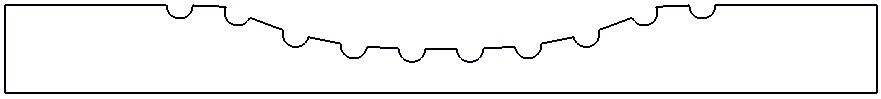
\includegraphics[scale=0.22]{./02_chaps/cap_solution/figure/CurvedStrut.png}\\
     (a) Curved Channel
     \end{center}
     \end{minipage}%
     \begin{minipage}{.45\linewidth}
     \begin{center}
      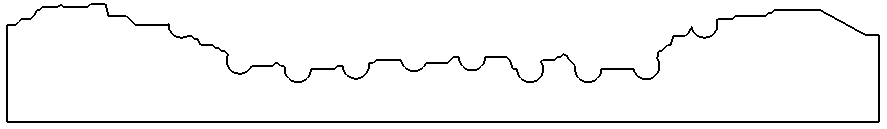
\includegraphics[scale=0.22]{./02_chaps/cap_solution/figure/RealStrut.png}\\
     (b) Real Channel
     \end{center}
     \end{minipage}\\[3mm]
     \end{center}
     \source Source: Wang et al. (2017) \cite{wang2017}
     \label{coronary artery geo}
\end{figure}
